\documentclass{acm_proc_article-sp}
\usepackage{booktabs}
\usepackage{url}
\usepackage{placeins}
\usepackage{listings}
\usepackage{multicol}
\usepackage{blindtext, subfig}
\usepackage{dblfloatfix} % fix for bottom-placement of figure

\lstset{breaklines=true}

\begin{document}

\title{Coevolution Between iAnts and Obstacles
\titlenote{The first project for CS 491 at The University of New Mexico}}

\numberofauthors{1}
\author{
\alignauthor
Troy M. Squillaci\\
       \affaddr{University of New Mexico}\\
       \affaddr{Department of Computer Science}\\
       \affaddr{Albuquerque, New Mexico}\\
       \email{zivia@unm.edu}
}

\maketitle

\begin{abstract}

This report presents results from investigating how autonomous robot ant swarms can forage for food in the presence of burdensome obstacles. In particular, I discuss how coevolution, manifested by a genetic algorithm, applies when evolving both ant behaviors and obstacle placements simultaneously. I demonstrate that an "ebb and flow" pattern emerges when these two populations of agents compete for dominance. Lastly I show that, given enough time, ant swarms tend to outperform obstacles due to their more diverse genome.

\end{abstract}

\section{Introduction}
The intention is to determine reactive behaviors that emerge from coevolving robot ant swarms and obstacles. Robot ant swarms each consist of a set of agents known as iAnts that are capable of mimicking the behaviors of live ants. Obstacles are agents consisting of immovable, fixed-size barriers. Both iAnt swarms and obstacles coexist in an environment known as an arena. The arena is composed of a finite space containing a centrally located nest and food tags uniformly distributed at random throughout.

The iAnt swarms are tasked with collecting as much food as possible within the environment. The behavior of an iAnt swarm is dictated by a foraging strategy defined by the parameters of a central-place foraging algorithm (CPFA). CPFA parameters are described in the Keywords section of this paper. The fitness of a swarms' foraging strategy, within a given environment, is calculated by $\frac{the\ amount\ of\ food\ collected}{the\ amount\ of\ food\ available}$.

The CPFA is an algorithm for autonomous swarm systems, which searches for and collects resources. An overview of the CPFA is given by Hecker\cite{hecker:CPFA}. See Figure \ref{fig:CPFA}.

\begin{figure*}[t]
	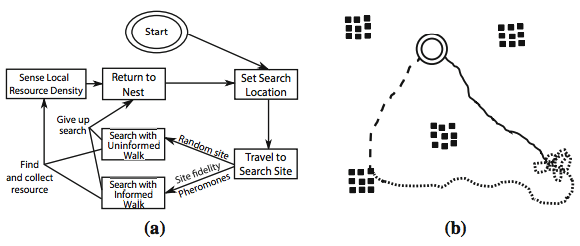
\includegraphics[width=18cm]{images/CPFA}
	\caption{(a) State diagram describing the flow of behavior for individual robots during an experiment. (b) An example of a single cycle through this search behavior. The robot begins its search at a central nest site (double circle) and sets a search location. The robot then travels to the search site (solid line). Upon reaching the search location, the robot searches for resources (dotted line) until a resource (square) is found and collected. After sensing the local resource density, the robot returns to the nest (dashed line)
	\cite{hecker:CPFA}} 
	\label{fig:CPFA}
\end{figure*}

Two important notions used in the CPFA are pheromones and site fidelity. Pheromones refer to invisible trails that the iAnts lay down when bringing food back to the nest. Pheromone trails can be discovered and followed by any iAnt. Therefore pheromone trails act as a recruiting device. They can direct other iAnts to points of interest such as food clusters and define navigable paths through sets of obstacles. Pheromone rate is the frequency at which pheromones are laid. Pheromone decay rate is how quickly pheromones evaporate. Site fidelity is a memory mechanism which iAnts use to travel back to previously discovered food sites. Site fidelity rate is the frequency at which site fidelity is utilized.

The obstacles are tasked with being as burdensome as possible by arranging themselves in clever ways to inhibit the foraging capabilities of the iAnts. A set of orientation-position (OP) vectors defines the placement of obstacles within the arena. The fitness of a set of obstacles is calculated by $1 - iAnt\ Swarm\ Fitness$.

Unlike the CPFA parameters which define foraging strategies for the collective whole of iAnt agents (the swarm), OP vectors are agent specific and thus differ between agents. The OP vectors used for current experiments are restricted such that only the $X$ element of the orientation vector and the $X,Y$ elements of the position vector are utilized. This is a deliberate choice aiming to reduce the search space since iAnts only navigate in two dimensions.

In this paper I examine the experiments, the results, and their significance. In particular, I report on the following:

\begin{itemize}
	\item Show that the nature of the two fitness functions leads to reactive behaviors between the two populations.
	\item How the obstacles form into notable patterns to exploit weaknesses of the CPFA.
	\item Explain advantageous qualities of iAnt swarms that allows them to overtake obstacles in long-running simulations.
\end{itemize}



\section{Results}

Below are the results and analysis of the tests. An important note, pheromone rate and site fidelity rate are defined by the range always[0.0, 20.0]never. This indicates that the magnitude of the value is inversely proportional with the utilization of its respective strategy. This is the definition in the iAnt extension of the ARGoS simulator. Additionally obstacles cannot physically be arranged to completely obstruct the nest. Finally agents are pitted against each other based on similar fitness values.



\subsection{Reactionary Elements} \label{sec:part1}

In this section I analyze how the definitions of the fitness functions lead to reactionary behaviors between the two populations of agents. Fitness functions serve as domain-specific quantifications for behaviors of agents. When multiple fitness functions coexist and promote competition between agents in the same domain, dynamic behaviors can emerge. This notion is demonstrated with the two fitness functions described above.

Notice that the fitness functions promote opposite outcomes, but use the same metric for their evaluations. In other words, iAnts swarms are rewarded for collecting more food tags while sets of obstacles are rewarded for preventing iAnts from collecting food tags.

An important feature of the fitness function for obstacles is that all agents initially have incredibly high fitness values. This is the exact opposite of the initial fitness values for the iAnts swarms. The result of this is that swarms are prompted to innovate and compete while obstacles have no incentive to do so since they already vastly outperform the competition.

This can be seen in Figure \ref{fig:iAntfitness20} and in Figure \ref{fig:obstaclefitness20}. The fitness of the iAnt swarms quickly rises as feasible foraging strategies are discovered. At around generation 5 it can be seen that reactionary behavior takes place as the obstacles adapt to the iAnt swarms raising in dominance.

\begin{figure}[h]
	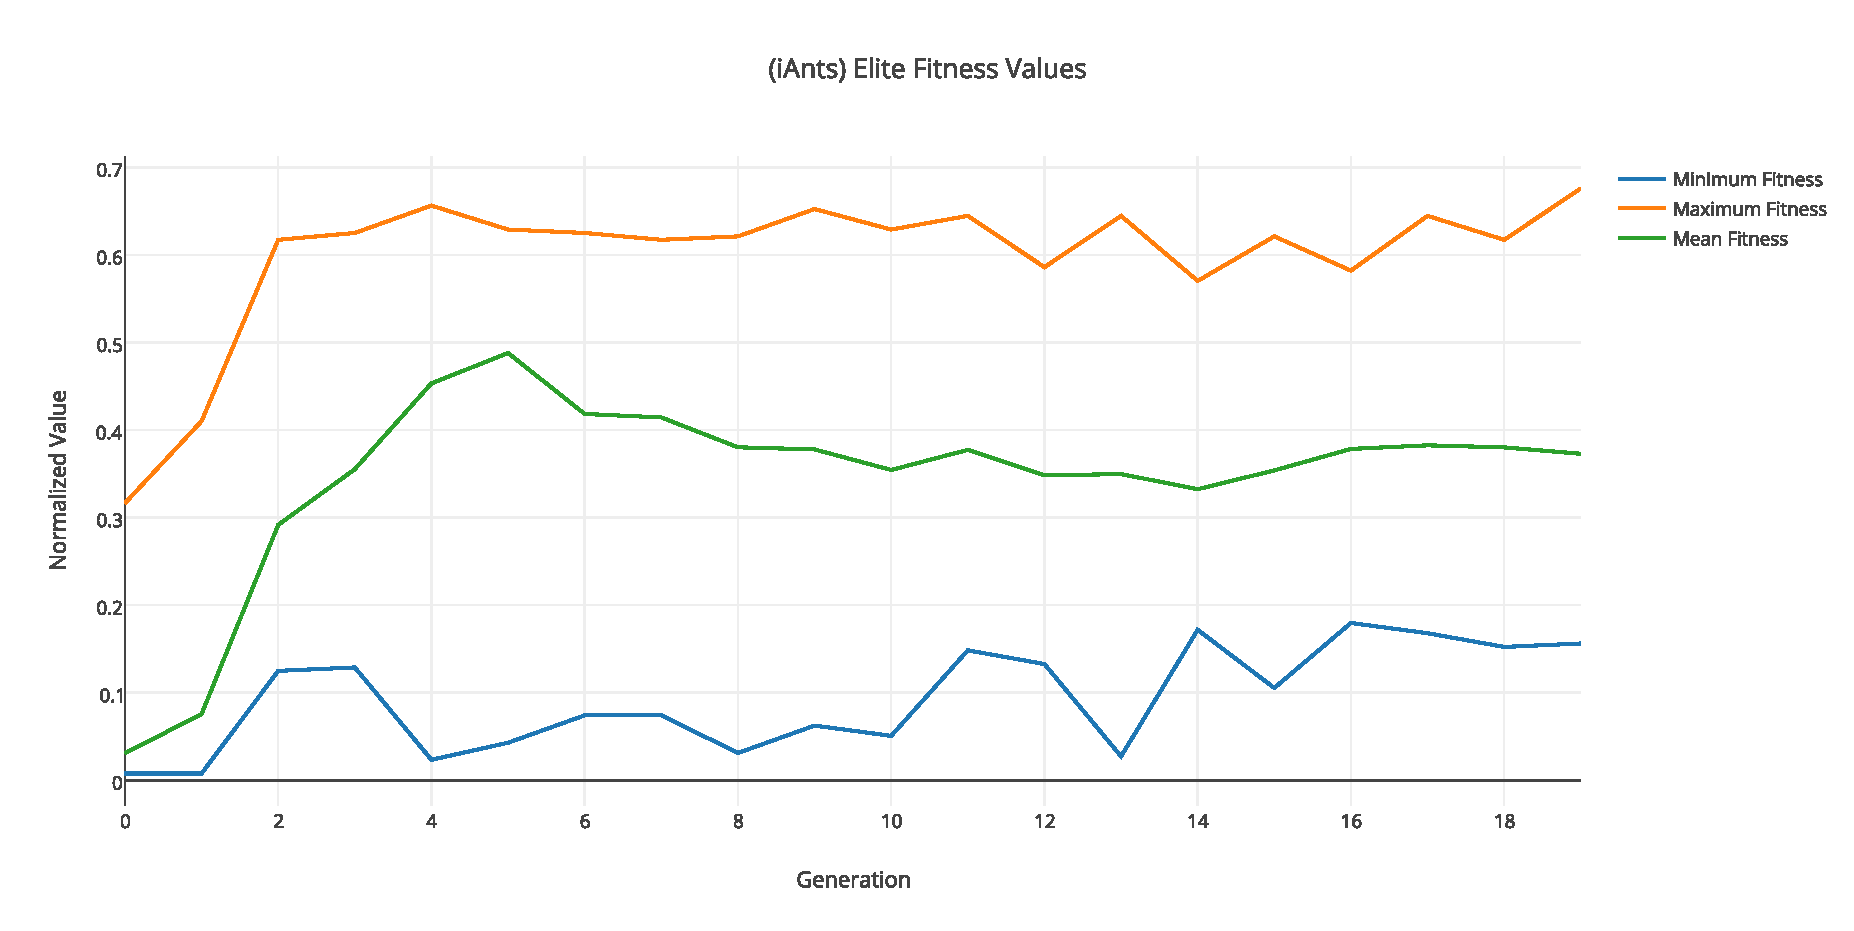
\includegraphics[width=9cm]{images/iAntsEliteFitnessValues20}
	\caption{The minimum, maximum, and mean fitness of the elite iAnt swarms population over 20 generations.} 
	\label{fig:iAntfitness20}
\end{figure}

\begin{figure}[h]
	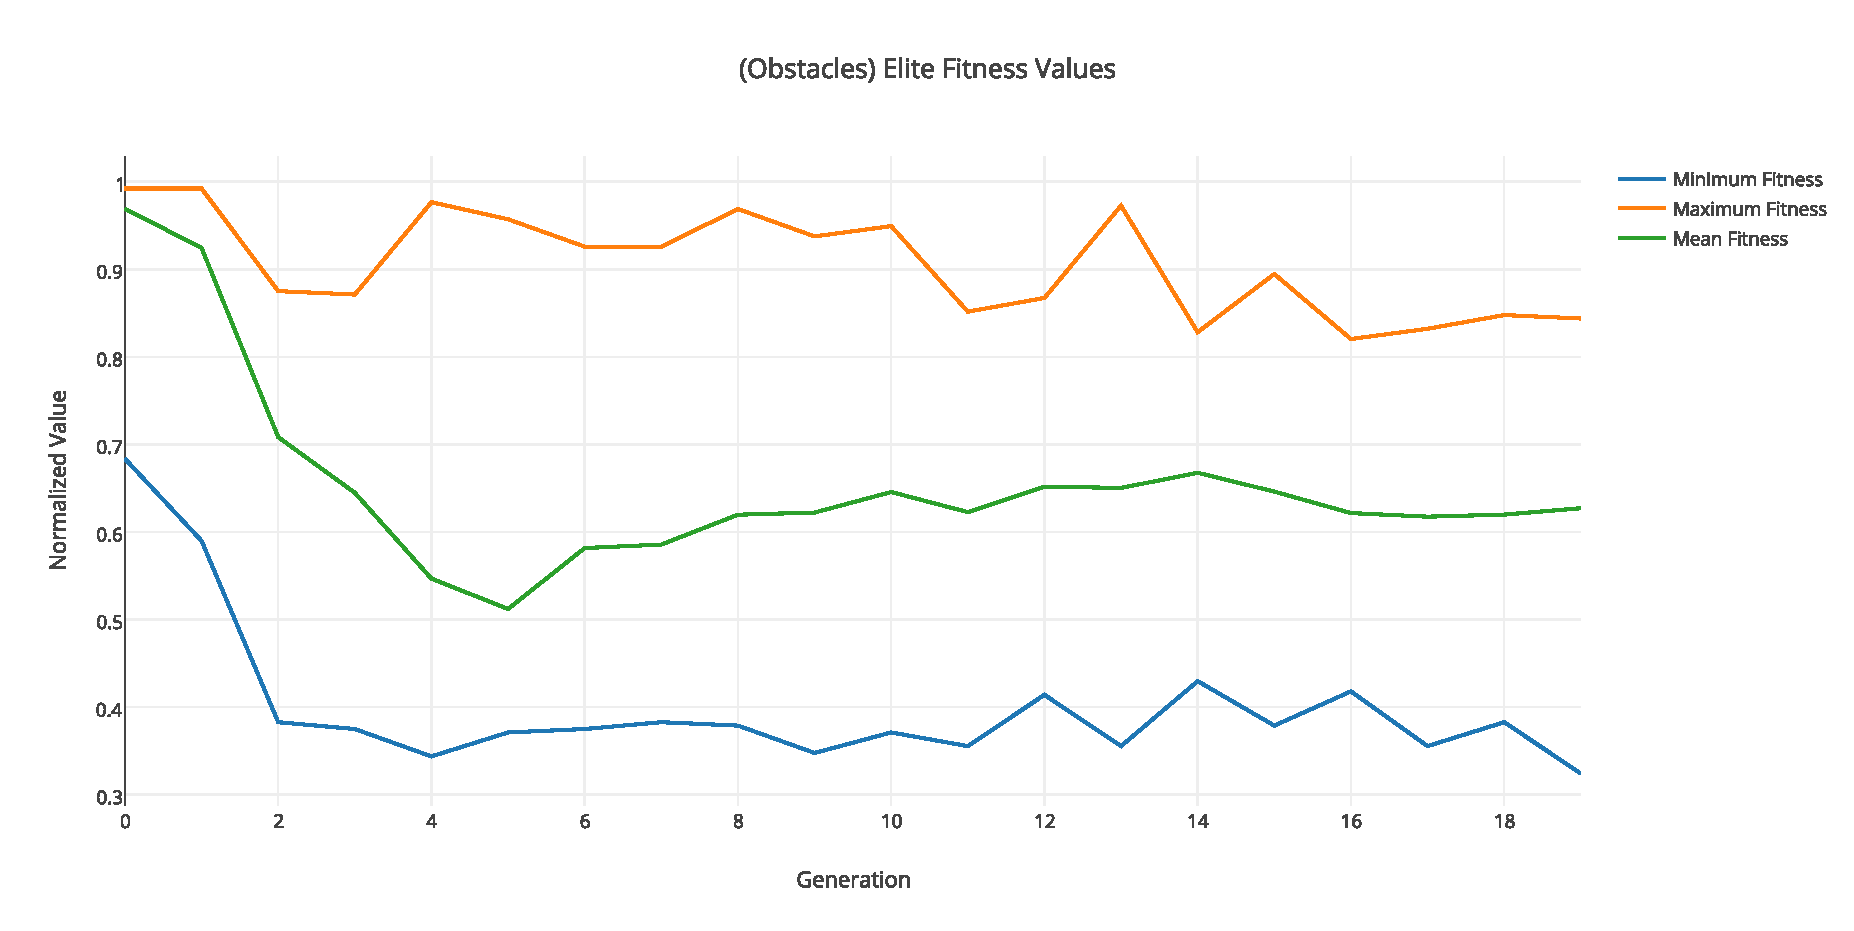
\includegraphics[width=9cm]{images/ObstaclesEliteFitnessValues20}
	\caption{The minimum, maximum, and mean fitness of the elite obstacle sets population over 20 generations.} 
	\label{fig:obstaclefitness20}
\end{figure}

Figure \ref{fig:obstaclemean20} shows the evolved mean of OP vectors for obstacles over 20 generations. Around half of the OP vector parameters diverged to cover areas closer to the nest which resulted in iAnt swarms encountering difficulties when attempting to leave or return to the nest.

\begin{figure}[h]
	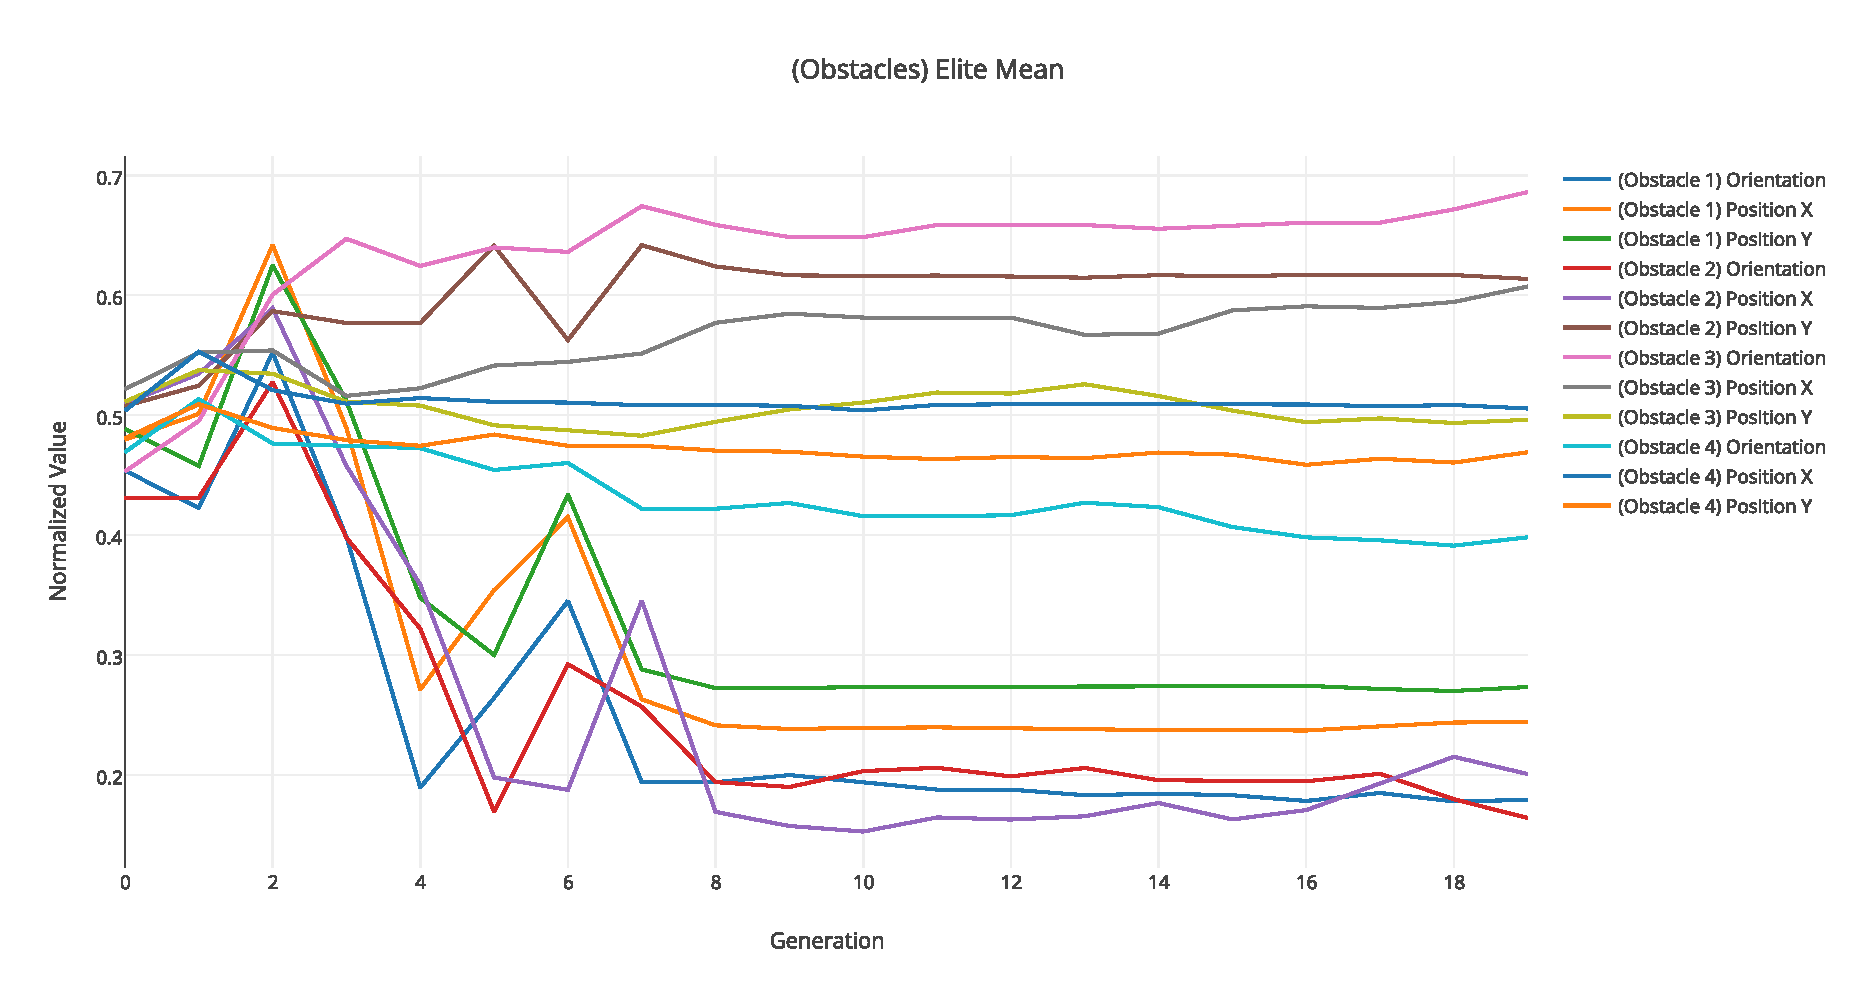
\includegraphics[width=9cm]{images/ObstaclesEliteMean20}
	\caption{The mean of OP vectors for elite obstacle sets over 20 generations.} 
	\label{fig:obstaclemean20}
\end{figure}



\subsection{Notable Obstacle Placements}

In this section I examine an unexpected and effective placement strategy for obstacles. This strategy listed here exploit a weaknesses of the CPFA in one form or another.

The strategy we analyze is one in which obstacles evolve to line up next to one another; forming a continuous wall-like structure. This can be seen in Figure \ref{fig:obs1}.

\begin{figure}[h]
	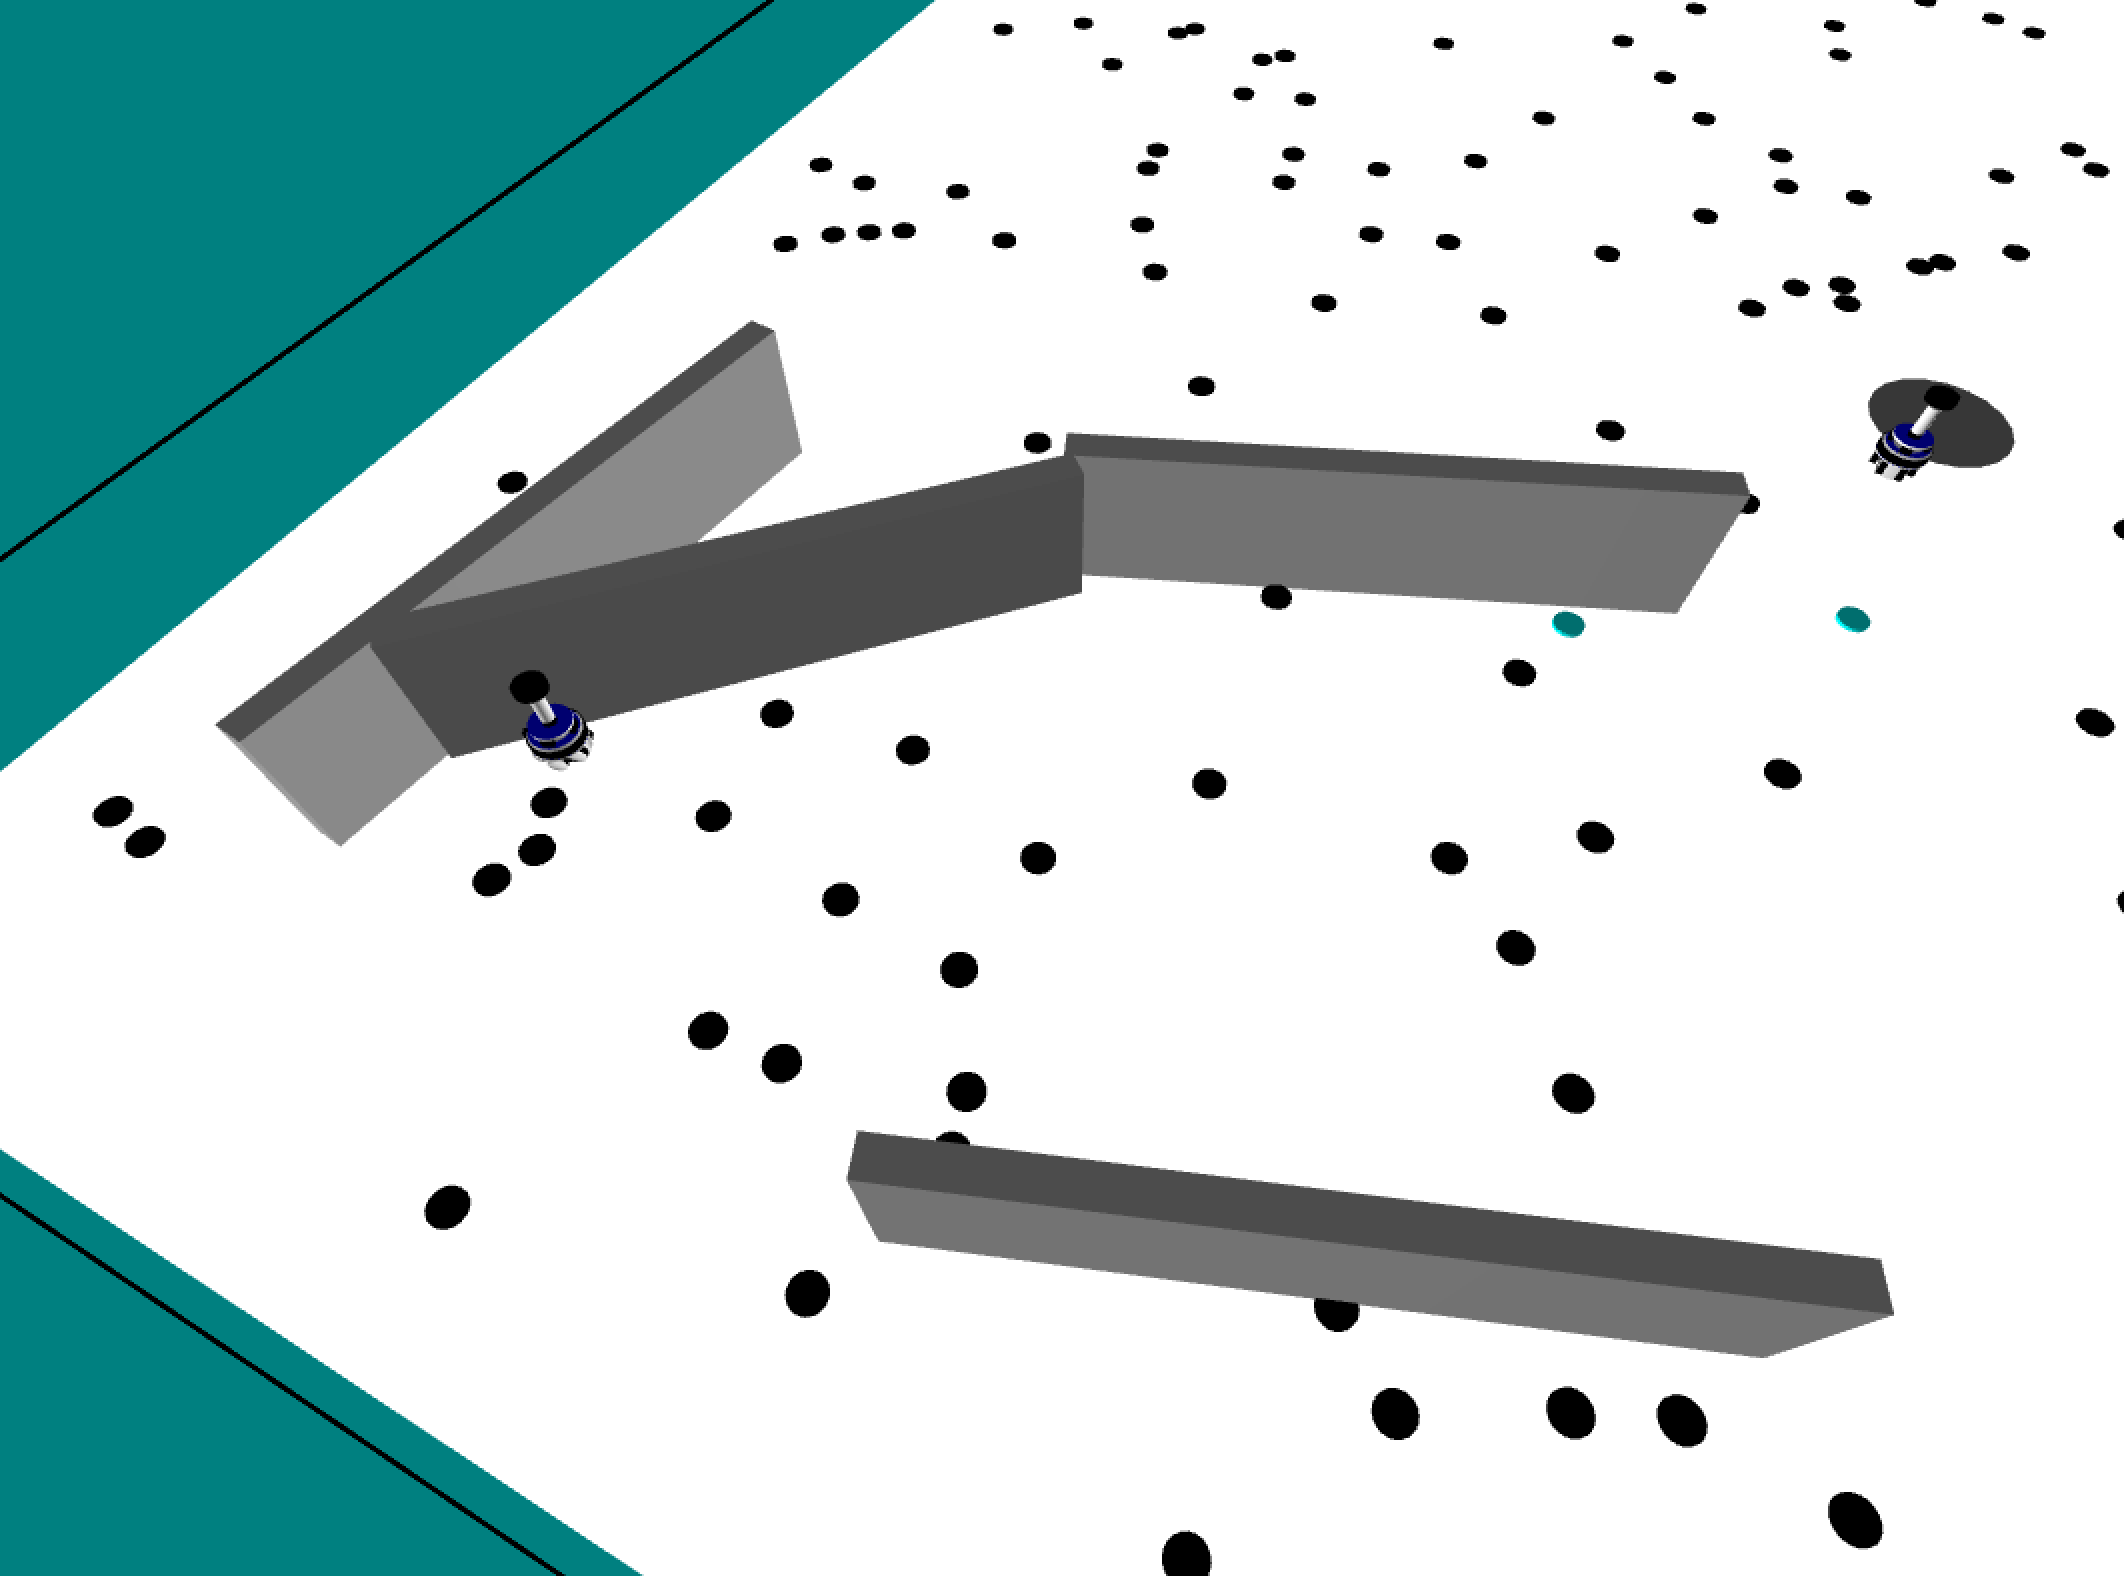
\includegraphics[width=9cm]{images/obs1}
	\caption{A continuous wall-like structure formed by obstacles exploiting iAnts attempting to return to the nest.} 
	\label{fig:obs1}
\end{figure}

This structure exploits how the CPFA handles movement to and from the nest. In particular, the uninformed search variation and probability of switching to searching parameters were likely much less effective. Additionally when an iAnt did discover food behind the wall, they usually became trapped due to the path-finding techniques used to return to the nest. They would often give-up and attempt to find another path but in most cases all paths they considered were obstructed. It seems that pheromones were more heavily utilized in such scenarios which allowed known valid pathways to be marked. 



\subsection{Long-Term Performance} \label{sec:obstacles}

This final section discusses long-running simulations covering up to twice as many generations as regular simulations. In almost all cases the iAnt swarms were able to vastly outperform the obstacles.

Consider the following simulation that covered 40 generations. This can be seen in Figure \ref{fig:iAntfitness40}. The iAnt swarms have a difficult time outperforming the obstacles for around the first 12 generations. However an innovative discovery is made which dramatically increases fitness over the next few generations. In Figure \ref{fig:iAntmean40} its clear that major changes took place that vastly altered the behavior of the swarms.

The CPFA provides higher genomic complexity than the current OP vectors for the obstacles. This leads to iAnt swarms being able to adapt in ways that allows them to navigate obstacles in different configurations. Parameters such as pheromones and uniformed search variations can be invaluable when tuned properly as they can assist in mitigating the effects of traps while at the same time have the ability to cover enough space to discover food in most areas of the arena.

\begin{figure}[h]
	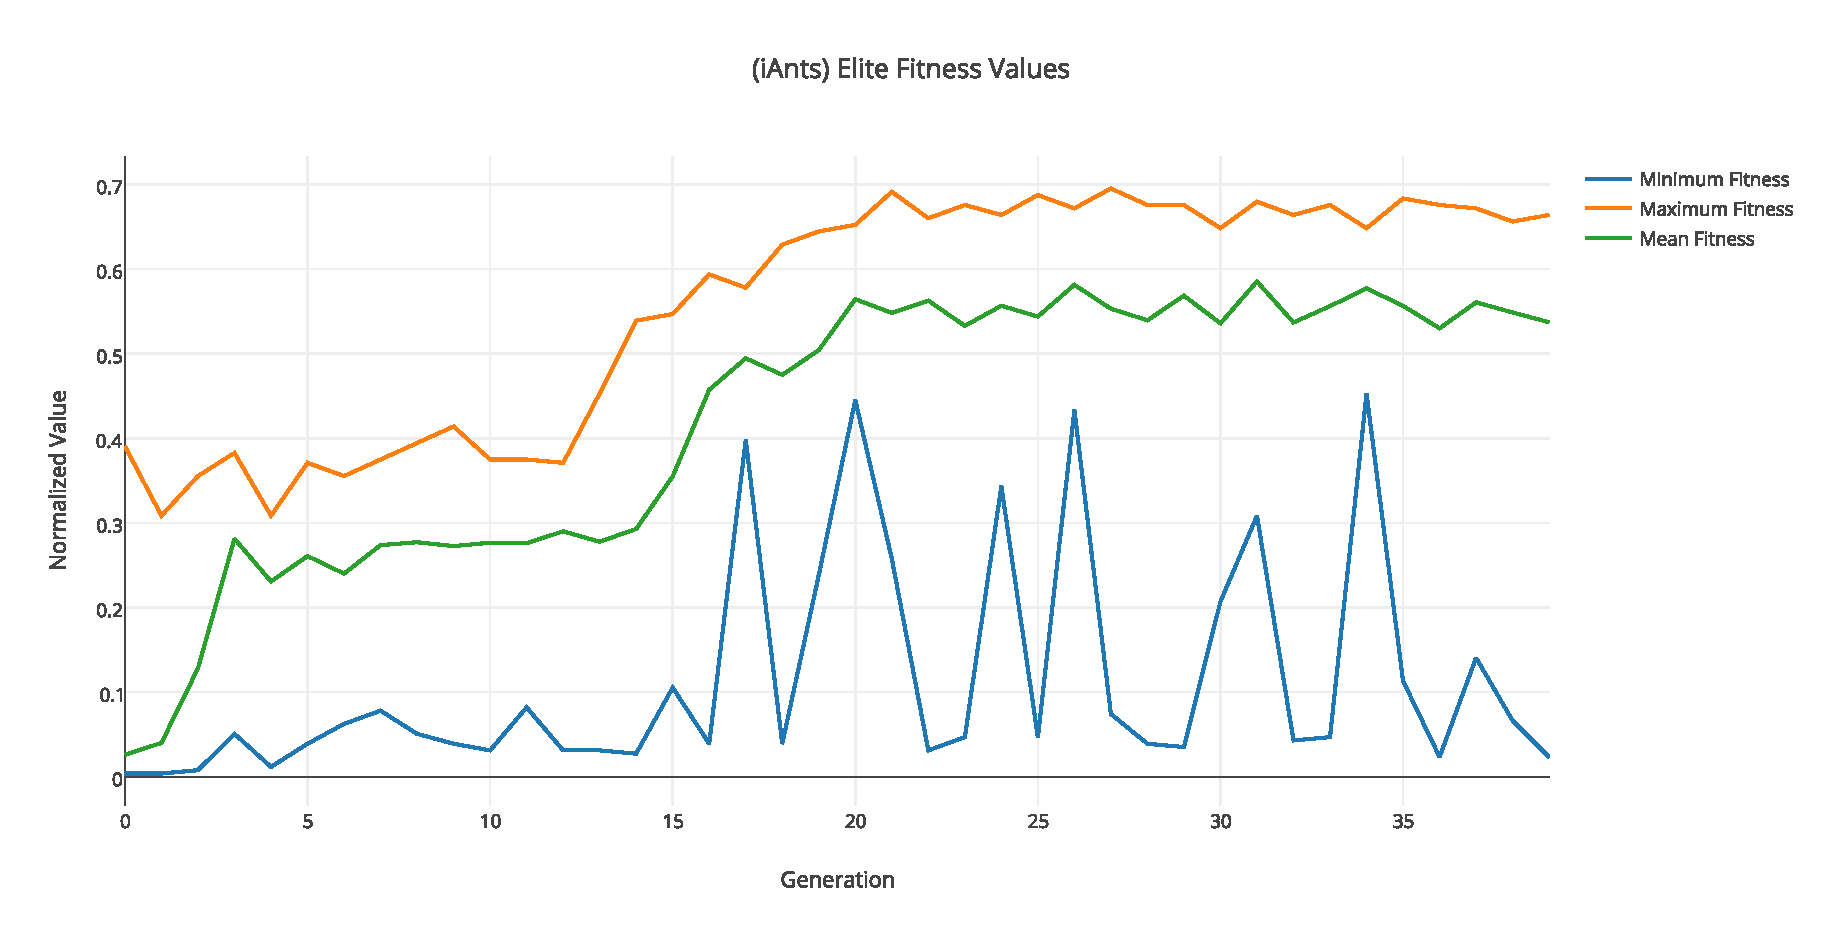
\includegraphics[width=9cm]{images/iAntsEliteFitnessValues40}
	\caption{iAnt swarms overtaking obstacles long-term.} 
	\label{fig:iAntfitness40}
\end{figure}

\begin{figure}[h]
	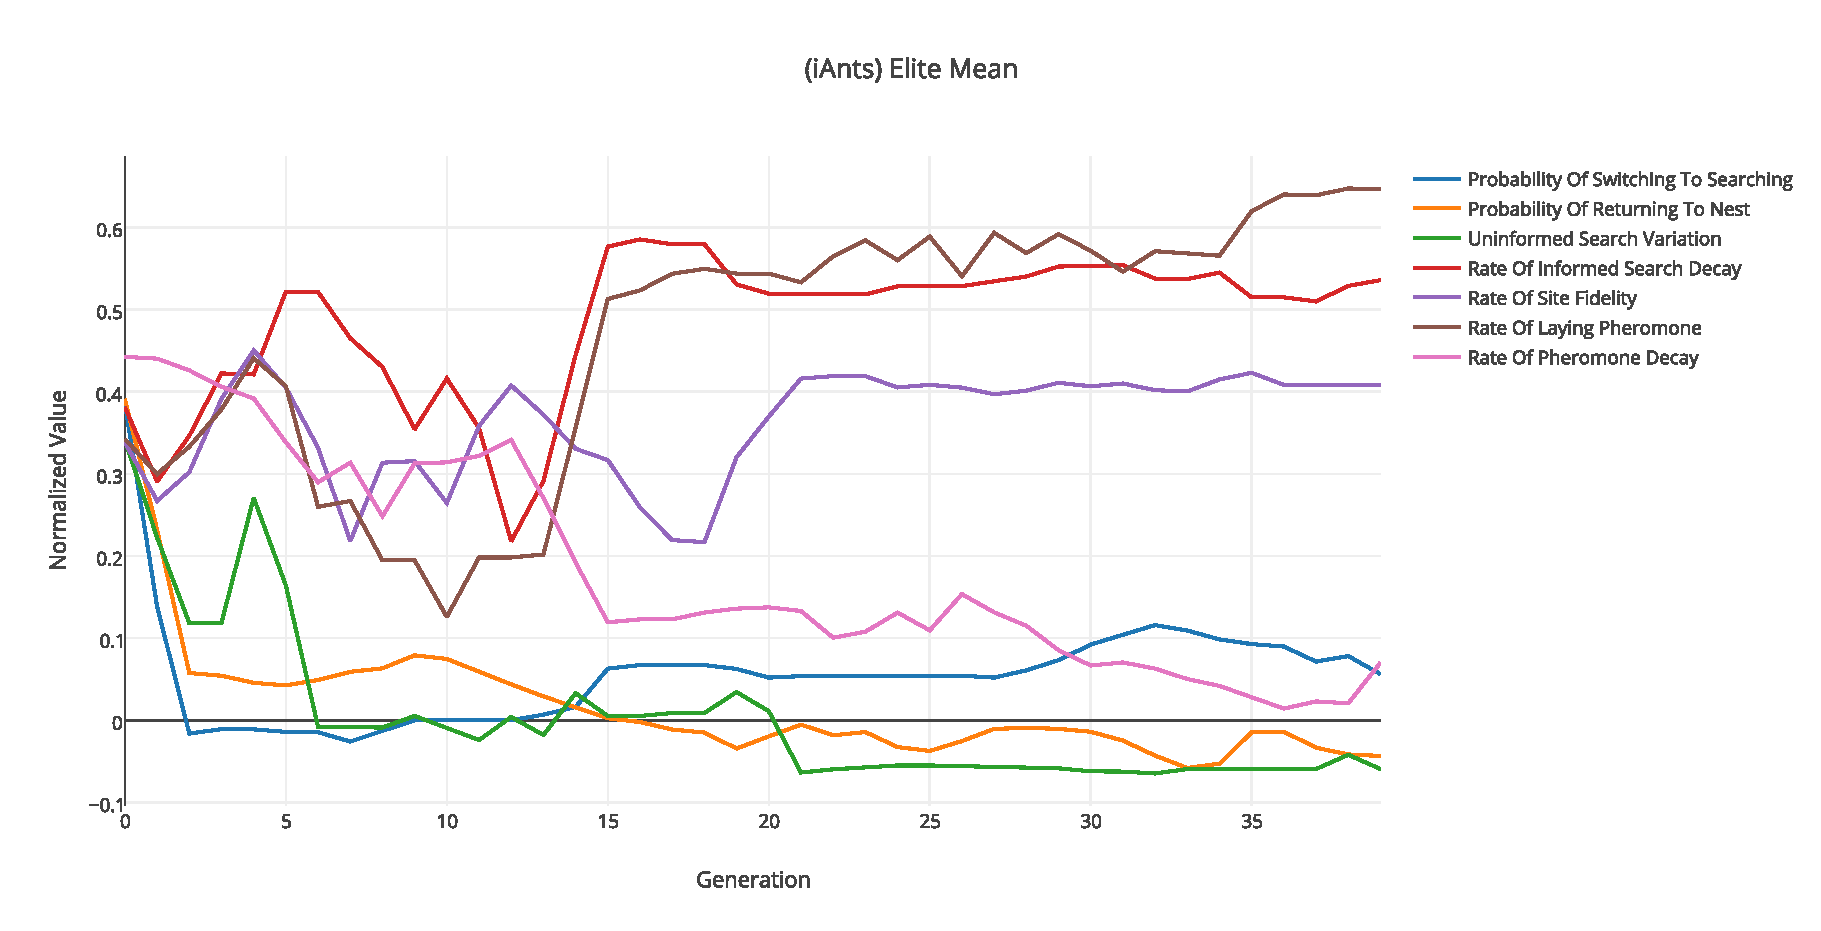
\includegraphics[width=9cm]{images/iAntsEliteMean40}
	\caption{iAnt swarms mean CPFA parameters for long-term simulation.} 
	\label{fig:iAntmean40}
\end{figure}

\keywords{
\textbf{GA: Genetic Algorithm} - An algorithm which generates each individual from some encoded form known as a "chromosome" or "genome". Chromosomes are combined or mutated to breed new individuals. "Crossover", the kind of recombination of chromosomes found in sexual reproduction in nature, is often also used in GAs. Here, an offspring's chromosome is created by joining segments chosen alternately from each of two parents' chromosomes which are of fixed length. GAs are useful for multidimensional optimization problems in which the chromosome can encode the values for the different variables being optimized.
\cite{Dictionary.com2015} \\

\textbf{CPFA:} Central-Place Foraging Algorithm\cite{iAntArgosWiki}
\begin{itemize}
	\item \textbf{PSS:} Probability Of Switching To Searching
	\item \textbf{PRN:} Probability Of Returning To Nest
	\item \textbf{USV:} Uninformed Search Variation
	\item \textbf{RISD:} Rate Of Informed Search Decay
	\item \textbf{RSF:} Rate Of Site Fidelity
	\item \textbf{RLP:} Rate Of Laying Pheromone
	\item \textbf{RPD:} Rate Of Pheromone Decay
\end{itemize}
}

\textbf{OP:} Orientation-Position Vector
\begin{itemize}
	\item \textbf{ORIX:} Orientation X Value - The X value of the orientation vector.
	\item \textbf{ORIY:} Orientation Y Value (Fixed) - The Y value of the orientation vector.
	\item \textbf{ORIZ:} Orientation Z Value (Fixed) - The Z value of the orientation vector.
	\item \textbf{POSX:} Position X Value - The X value of the position vector.
	\item \textbf{POSY:} Position Y Value - The Y value of the position vector.
	\item \textbf{POSZ:} Position Z Value (Fixed) - The Z value of the position vector.
\end{itemize}

\section{Discussion}

One of the most challenging aspects of this project was determining how to define the fitness functions. The overarching goal was to encourage competition between two coevolved populations of agents in hopes of discovering interesting reactions. The fitness functions are incredibly important components in manifesting such reactions. I suspect that the definitions of the fitness functions listed here may not be ideal. I've considered including simulation time as a variable in calculating fitness, but I am avoiding overcomplicating them in hopes of avoiding deceptive results.

Future plans for this project include introducing variable-sized obstacles and stationary food piles (with a clustered distribution and a constant seed value between simulations). Doing so may lead the iAnt swarms and obstacles to determine the location of the food clusters prior to the simulations even starting. In such cases obstacles may have significant advantages over the iAnts since they would be able to localize obstructions around the most dense piles of food. 

Additionally I would like to investigate if substantially different placements strategies for obstacles would arise when more obstacles are added to the arena. I feel that this is a double-edged sword. Unlike iAnt swarms which rely on a single CPFA parameter list for the entire swarm, obstacles each have their own OP vector set. Therefore introducing more obstacles increases the complexity of the collective genome of the obstacles. This would allow for more elaborate placement strategies but would also vastly increase the search space which could be detrimental in shorter running simulations.

\section{Methods}
This section details the methods used to conduct the experiments.

\subsection{Genetic Algorithm}

\begin{table}[h]
\begin{tabular}{@{}ll@{}}
\toprule
Parameter              & Value      \\ \midrule
Population Size        & 40         \\
Elite Size             & 8          \\
Generations            & 20-40         \\
Mutational Probability & 10\%       \\
Simulation Duration    & 30 Minutes \\
Number of Food Tags    & 256        \\ 
Number of iAnts        & 6          \\ 
Number of Obstacles    & 4          \\ \bottomrule
\end{tabular}
\caption{Shows the exact parameters used for the GA.}
\label{table:gaParams}
\end{table}

The GA begins by initializing a population of iAnts swarms and obstacles. Initialization consists of forming a set of CPFA parameters for each iAnt swarm and a set of OP vectors for obstacles. Both of these parameter sets are uniformly distributed over [0, 1] (scaled) with offsets determined by sampling a normal distribution.

Lower and upper bounds are imposed on both the CPFA parameters and OP vectors to reduce the search space and exclude what are deemed as infeasible solutions. Such bounds are determined on a case-by-case basis; usually discovered by trial and error.

\begin{table}[h]
\begin{tabular}{@{}lll@{}}
\toprule
Parameter & Lower Bound & Upper Bound \\ \midrule
PSS       & 0.0         & 1.0         \\
PRN       & 0.0         & 1.0         \\
USV       & 0.0         & 180.0       \\
RISD      & 0.0         & 1.0         \\
RSF       & 0.0         & 20.0        \\
RLP       & 0.0         & 20.0        \\
RPD       & 0.0         & 1.0         \\ \bottomrule
\end{tabular}
\caption{The upper and lower bounds imposed on CPFA parameters.} \label{table:cpfaBounds}
\end{table}

\begin{table}[h]
\begin{tabular}{@{}lll@{}}
\toprule
Parameter    & Lower Bound & Upper Bound \\ \midrule
ORIX         & 0.0         & 90.0        \\
ORIY (Fixed) & 0.0         & 0.0         \\
ORIZ (Fixed) & 0.0         & 0.0         \\
POSX         & 1.5         & 5.0         \\
POSY         & 1.5         & 5.0         \\
POSZ (Fixed) & 0.0         & 0.0         \\ \bottomrule
\end{tabular}
\caption{The upper and lower bounds imposed on OP vectors.} \label{table:opBounds}
\end{table}

A random seed is generated for each simulation, then simulations are dispatched to a process pool and asynchronously executed. When simulations complete, their respective fitnesses for both iAnts swarms and obstacles are calculated. Control returns to the GA once all simulations have completed. At the end of each generation, elite individuals in the 80th percentile of both iAnt swarm and obstacle populations are chosen based on fitness. Remaining individuals are reformed by means of one-point crossover between randomly chosen individuals in the elite population followed by gaussian mutation. Each CPFA parameter and OP vector has a 10\% chance to undergo mutation. Mutation is determined by taking a sample from a normal distribution with a mean equal to the current value of the parameter and a scaled standard deviation of 0.05. The scaling of the standard deviation relative to CPFA and OP vector bounds appears to prevent premature convergence to local optima. Reactive behavior between the iAnt swarms and obstacles takes time to manifest do to the nature of the fitness function. Therefore the GA must run long enough to see such emergent behaviors - typically 20-40 generations is sufficient.

\subsection{Analysis Method}

Python's "multiprocessing" module provided the capability of asynchronously distributing simulations across available processing cores which led to massive performance improvements. Simulations are performed in a large-scale autonomous robot simulator - ARGoS. Additionally, extensive usage of the Python modules "numpy" and "plotly" allowed data collection, analysis, and visualization to be performed with ease. All other segments of the program such as the GA were also written in Python.


% The following two commands are all you need in the
% initial runs of your .tex file to
% produce the bibliography for the citations in your paper.
\bibliographystyle{abbrv}
\bibliography{Troy-Squillaci-Project1}
%\balancecolumns
\appendix
\section{Plot.ly Page}\label{sec:one}
Plots shown in this paper can be viewed at https://plot.ly/$\sim$Zivia\section{Bitbucket Page}\label{sec:two}
The code repository can be found at https://bitbucket.org/Zivia/gw2-evolution. This is a private repository. To gain access you must be added as a contributor. Contact the author to be added.

\end{document}